\section{Polyline Simplification in \(\R^1\)}\label{sec:dimension_one}
In this section, we investigate the global and local simplifications in one dimension. We show that they always have the same size when using the Fréchet distance and thus local simplification algorithms can be used. Finally, we outline a linear algorithm to solve the simplification problem. We also consider various Hausdorff variants. This shows that \citeauthor{polyline_simplification_has_cubic_complexity_bringmannetal}'s conditional lower bound can be broken in lower dimensions. After this, we also consider different distance metrics to measure simplification against polylines.

We identify each point with a value on the real line. We associate the negative direction with with left and the positive with right. Throughout this whole section, let \(P = \angl{u_0, \dots, u_n}\) be a polyline with \(n\) line segments and \(\varepsilon \geq 0\).

\subsection{Related Works}
The case of one dimensional polyline simplification has been considered less often than the two dimensional case or the general case. The known optimal results are aware of include \citeauthor{global_curve_simplification}~\cite{global_curve_simplification} which show that curve-restricted global Fréchet simplification simplification can be solved in linear time, and \citeauthor{min_complexity_1d_unrestricted}\cite{min_complexity_1d_unrestricted} show that the unrestricted Fréchet setting can be solved in linear time. The other settings were not considered and \citeauthor{global_curve_simplification} do not mention any one dimensional results for other settings. 

A linear time algorithm was found by \citeauthor{clustering_time_series}~\cite{clustering_time_series} that is optimal for all five settings, their algorithm is suboptimal \emph{only if} the problem definition allows dropping the start and end points. Under the definitions by \citeauthor{global_curve_simplification}, their algorithm is optimal. This clear distinction could be the reason that this result is less known.

We present alternative, visual proofs for the Fréchet cases from the perspective of polyline simplification and also cover the Hausdorff cases. The algorithms we provide are very similar to the curve-restricted algorithm from \citeauthor{global_curve_simplification} with minor modifications and equivalent to the one by \citeauthor{clustering_time_series}. This serves as a summary of known results in \(\R^1\).

\subsection{Restricted Fréchet Distance}
We show that every local vertex-restricted simplification is also global curve-restricted solution. Among the four variants (local vertex-restricted, local curve-restricted, global vertex-restricted, and global curve-restricted) these two variants always have the largest and smallest simplification sizes respectively and thus, we show that in one dimension all four variants can be solved in the same way.

\begin{observation}
	All point distances \(\delta\) coincide in \(\R^1\) with \(\delta(u, v) = |u-v|\). We will therefore not mention any specific distance \(\delta\).
\end{observation}

\begin{lemma}[Zigzag]\label{lem:zigzag}
  Let \(Q = \angl{u_{i_0}, \dots, u_{i_k}}\) be a local or global simplification of \(P\) and \(u_{i_{j-1}}\), \(u_{i_{j}}\), and \(u_{i_{j+1}}\) be three consecutive vertices on the simplification. Then either
	\begin{itemize}
	  \item \(u_{i_{j-1}} < u_{i_{j}}\), and \(u_{i_{j}} > u_{i_{j+1}}\), or 
	  \item \(u_{i_{j-1}} > u_{i_{j}}\), and \(u_{i_{j}} < u_{i_{j+1}}\).
	\end{itemize}

	This means that both local and global simplifications always alternate between going left and going right.
\end{lemma}

\begin{proof}
  It is trivial that no two consecutive points can be the same as we could simply remove one of the two points that share the same position since the shortcut between those points has length 0 (also holds in higher dimensions). 

	Assume that \(u_{i_{j-1}} < u_{i_{j}}\) and \(u_{i_{j}} < u_{i_{j+1}}\), i.e., the simplification goes right twice. By skipping the middle point, the resulting shortcut from \(u_{i_{j-1}}\) to \(u_{i_{j+1}}\) has Fréchet distance within \(\varepsilon\) with the concatenation of the two previously underlying polylines because the new shortcut is the concatenation of the previous two shortcuts. This new simplification has fewer vertices. Thus, the previous one was not optimal. The other case follows analogously. 
\end{proof}

\begin{theorem}[Restricted Fréchet Simplifications in \(\R^1\)]\label{thm:restr_frechet_1}
	Let \(P\) be a one dimensional polyline. Any (minimal) local vertex-restricted simplification is also a (minimal) global curve-restricted simplification. Thus, the sizes of minimal simplifications of the four restricted variants (local vertex-restricted, local curve-restricted, global vertex-restricted, and global curve-restricted) coincide.
\end{theorem}

\begin{proof}
	If only one shortcut suffices in the global case, it must be between the start and end which is a local vertex-restricted simplification. Thus we assume there are at least two shortcuts in the global curve-restricted simplification.

	Let \(Q\) be a global curve-restricted simplification. We iteratively modify \(Q\) to obtain a local vertex-restricted simplification. We consider the first pair of successive shortcuts \(e = \overline{P(i)P(j + \gamma)}\) and \(e' = \overline{P(j+\gamma)P(t)}\) and the underlying subpolylines \([a, b]\) and \([b, c]\) such that \(a = i\). Here, \(\gamma \in [0, 1]\), \(i\) and \(j\) are indices of vertices on the polyline and thus integers and \(t \in [0, n]\) can lie on the curve. Note that initially \(a = i = 0\) and as we iteratively update the shortcuts to match the end (which is the start of \(e'\)), we maintain this local start property for the shortcut throughout. Without loss of generality, assume that \(e\) goes right and \(e'\) goes left using \cref{lem:zigzag} and potentially mirroring the whole subpolyline.

	By definition, for the shortcuts and the underlying subpolylines, we get \(\delta^F(P[i \dots b], \overline{P(i)P(j + \gamma)}) \leq \varepsilon\) and \(\delta^F(P[b \dots c], \overline{P(j+\gamma)P(t)}) \leq \varepsilon\). We replace \(P(j + \gamma)\) with a new vertex \(P(j')\) and show that \(\overline{P(i)P(j')}\) is local and \(\delta^F(P[j' \dots c], \overline{P(j')P(t)})  \leq \varepsilon\). Thus, we maintain a curve-restricted simplification where increasingly all global curve-restricted shortcuts are replaced with local vertex-restricted shortcuts. Finally, we obtain a local vertex-restricted simplification with the same amount of vertices.

	Let \(P(j')\) be the rightmost vertex in \(P([i \dots c] \cap [i, t])\) (i.e., the part of the total subpolyline that lies between \(i\) and \(t\)). We need to show 
	\begin{enumerate}
		\item \(i < j' < t\) to maintain monotonicity of the simplification points,
		\item \(\delta^F(P[i \dots j'], \overline{P(i)P(j')}) \leq \varepsilon\), and
		\item \(\delta^F(P[j' \dots c], \overline{P(j')P(t)}) \leq \varepsilon\).
	\end{enumerate}

	\paragraph{Statement 1} We need to show that \(j'\) even exists. If no point on \(P[i \dots c]\) lies to the right of \(P(i)\) and \(P(t)\) then the shortcut \(\overline{P(i)P(t)}\) covers the whole subpolyline \([i, c]\) because going right of both \(P(i)\) and \(P(t)\) to \(P(j + \gamma)\) is useless resulting in a smaller simplification. If the first point right of both is after \(P(t)\) then the first shortcut cannot go right because \(i < j + \gamma < t\) unless \(P(i) \leq P(j+\gamma) \leq P(t)\) which is two right-going shortcuts which cannot be. Thus, there is a point (not necessarily a vertex) right of both \(P(i)\) and \(P(t)\) on \(P[i \dots c]\). 

	Next, we claim that actually there is even a vertex, not just a point with these properties. The only possibility that this would be false is if the first vertex to the right of \(P(i)\) and \(P(t)\) is \(\lceil{c}\rceil\). In this case, as \(P(\lfloor{c}\rfloor) \leq P(t) \leq P(\lceil{c}\rceil)\) there is a point \(c' \in [\lfloor{c}\rfloor, c]\) with \(P(c') = P(t)\). We replace both shortcuts with \(\overline{P(i)P(t)}\) and update the subpolyline to \([i, c']\) and the following subpolyline from \([c, d]\) to \([c', d]\) resulting in a smaller potential simplification. We now demonstrate that this replacement indeed yields a valid simplification with fewer non-vertex points, contradicting the minimality of the original simplification. For the new shortcut, this is trivial as \([i, c'] \subseteq [i, c]\) and \(\delta(P(c'), P(t)) = 0 \leq \varepsilon\), and no point is right of both \(P(i)\) and \(P(t)\) thus going to \(P(j+\gamma)\) is unnecessary. For the following shortcut we note that it is a right-going shortcut as we have replaced a right-going and a left-going with a new shortcut so the following one must also go right. We use the same way to traverse the shortcut and subpolyline as the shortcut actually used but prepend going from \(P(c')\) to \(P(c)\) on the subpolyline which is possible as they lie on the same line segment, \(c' < c\), and the shortcut goes in the same direction as this line segment. Thus, we again obtain a contradiction to shortcut minimality of simplifications.

	Thus, we can actually assume that there is a vertex in \(P([i \dots c] \cap [i, t])\) that is right of both \(P(i)\) and \(P(t)\), and thus, \(j'\) is well-defined as in \([i, t] \cap [i, c]\) there are vertices and as the rightmost vertex among those is right of both \(P(i)\) and \(P(t)\) it cannot be either point and thus \(i < j' < t\).


	\paragraph{Statement 2 and 3}
	We distinguish two cases based on the relative order of \(b\) and \(j'\) on the polyline. In the case \(j' \leq b\), the first statement is easier to prove, while the second statement is simpler in the case \(j' < b\). We provide figures to visualize the cases. The polyline segment \([i, c]\) is marked in red, vertical differences are only used to compare the \(b\) and \(j'\) (a later index corresponds to a higher position) as well as to make the figures more readable.
	
	\paragraph{Case 1: \(j' \leq b\)}
	Refer to \cref{fig:case1}. There is a point \(P(i) \leq x \leq P(j + \gamma)\) on \(e\) such that \(\delta^F(P[i \dots j'], \overline{P(i)x}) \leq \varepsilon\) and \(\delta^F(P[j' \dots b], \overline{xP(j+\gamma)}) \leq \varepsilon\). it must be \(x \leq P(j')\) because \(P(j')\) is rightmost in \([i, j']\) trivially so no other point on \([i, j']\) forces \(x\) to go right of \(P(j')\) (or even \(P(j') - \varepsilon\)) so we can just traverse the local shortcut fully as \(P(j')\) is right of every vertex in the range and thus the remaining shortcut must cover everything up to \(P(j')\). 

	for the third statement, we use \(\delta^F(P[b\dots c], \overline{P(j+\gamma)P(t)}) \leq \varepsilon\). 

	\begin{figure}[b]
		\centering
		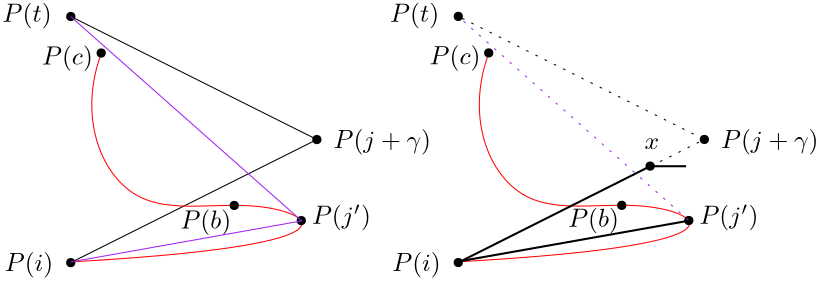
\includegraphics[scale=0.3]{./figures/case1.png}
		\caption{Case 1. Showing \(\delta^F(P[i \dots j'], \overline{P(i)P(j')}) \leq \varepsilon\) using \(\delta^F(P[i \dots j'], \overline{P(i)x}) \leq \varepsilon\) and \(P(j') - \varepsilon \leq x \leq P(j')\).}
		\label{fig:case1}
	\end{figure}

	\paragraph{Case 1.1: \(P(b) > P(j')\)} 
	Refer to \cref{fig:case11}. In this case \(b\) and \(c\) lie on the same line segment (otherwise both ends of the line segment on which \(b\) lies are contained in the subpolyline and thus considered in the definition of \(j'\)) which must go right (because the start of the line segment cannot be the right vertex of the line segment because \(P(b) > P(j')\)). We modify the subpolylines such that \(P(b') = \min(P(j+\gamma) - \varepsilon, P(\lfloor b \rfloor))\), i.e., the leftmost point on the line segment that is within \(\varepsilon\) of \(P(j+\gamma)\). This new point \(P(b')\) is still within \(\varepsilon\) of \(P(j+\gamma)\) by construction, so the condition \(\delta^F(P[b' \dots c], \overline{P(j+\gamma)P(t)}) \leq \varepsilon\) still holds. This satisfies \(P(b') \leq P(j')\) (if \(P(b')\) is the start of the line segment, it is used in the definition of \(j'\). If \(P(b') = P(j+\gamma)-\varepsilon\) it is left of \(P(j')\) as \(P(j')\) is within \(\varepsilon\) of \(P(j+\gamma)\)) and it still holds \(j' \leq b'\) thus we have not violated the previously proven first statement. With these modifications, we can use Case 1.2.

	\begin{figure}[b]
		\centering
		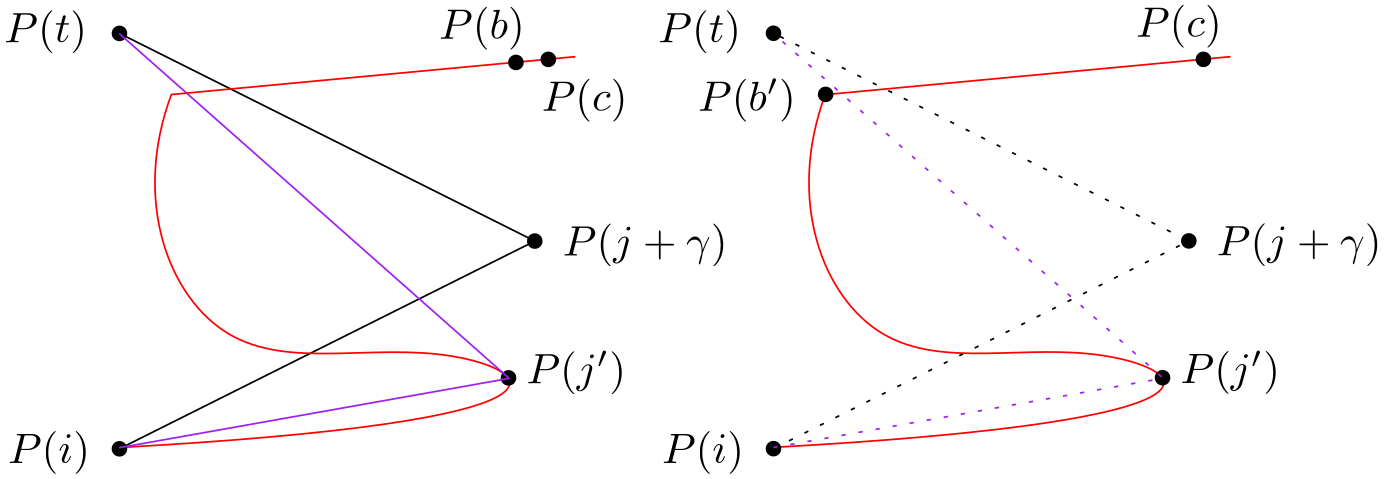
\includegraphics[scale=0.15]{./figures/case1-1.png}
		\caption{Case 1.1. Modifying \(b\) to \(b'\) such that it satisfies \(P(b') \leq P(j')\).}
		\label{fig:case11}
	\end{figure}

	\paragraph{Case 1.2: \(P(b) \leq P(j')\)} 
	Refer to \cref{fig:case12}. As \(P(j')\) is right of \(P(b)\) (and thus the whole subpolyline \([i, b]\)) we can use the shortcut \(\overline{P(j')P(t)}\) to go left by at most \(\varepsilon\) until we have traversed the subpolyline \([j', b]\) (if there are points further left than \(P(t)-\varepsilon\) between \(j'\) and \(b\) and \(P(j')-P(t) \leq \varepsilon\) then everything on \([i, c] \cap [i, t]\) can be covered by the direct shortcut \(\overline{P(i)P(t)}\)). Then we can use the traversal from \(\overline{P(j+\gamma)P(t)}\) for \([b, c]\) to traverse the rest. No point on the subpolyline requires a point on the shortcut right of \(P(j')\) (or even \(P(j') - \varepsilon\)) by construction, thus, even if \(P(j + \gamma)\) is further right than \(P(j')\) it does not yield reachable points that are unreachable using \(P(j')\) so we can imagine going left until we reach the point where we stopped on \(\overline{P(j')P(t)}\). If \(P(j+\gamma)\) is left of \(P(j')\), we first go left on \(\overline{P(j')P(t)}\) until we reach \(P(j+\gamma)\) (note that \(|P(j+\gamma) - P(j')| < \varepsilon\) as \(P(j+\gamma)\) is the right end of the previous shortcuts and must match \(P(j')\)).

	\begin{figure}[b]
		\centering
		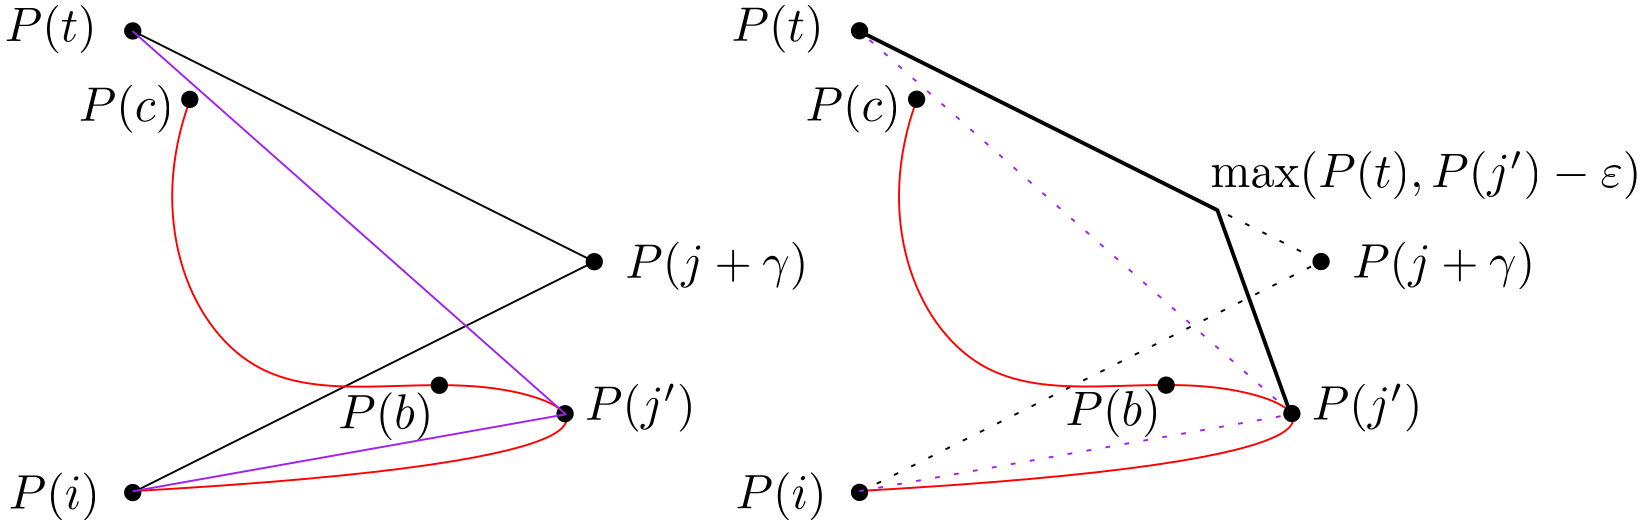
\includegraphics[scale=0.15]{./figures/case1-2.png}
		\caption{Case 1.2. Showing \(\delta^F(P[j' \dots c], \overline{P(j')P(t)}) \leq \varepsilon\) using \(\delta^F(P[b \dots c], \overline{P(j+\gamma)P(t)}) \leq \varepsilon\) and \(\delta^F(P(j') - \varepsilon, P[j' \dots b]) \leq \varepsilon\).}
		\label{fig:case12}
	\end{figure}

	\paragraph{Case 2: \(j' > b\)}
	Refer to \cref{fig:case2}. We first consider the last statement. To construct a traversal of \([j', c]\) while traversing the shortcut \(\overline{P(j')P(t)}\) we use that there is an \(x\) on the shortcut \(\overline{P(j+\gamma)P(t)}\) that witnesses \(\delta^F(P[j', c], \overline{xP(t)}) \leq \varepsilon\). Similar to Case 1, we can assume that \(x \leq P(j')\) as nothing forces \(x\) to be further right. We can thus traverse the shortcut until \(x\) while not moving on the shortcut and from there we use the traversal from \(\overline{P(j+\gamma)P(t)}\).

	\begin{figure}[b]
		\centering
		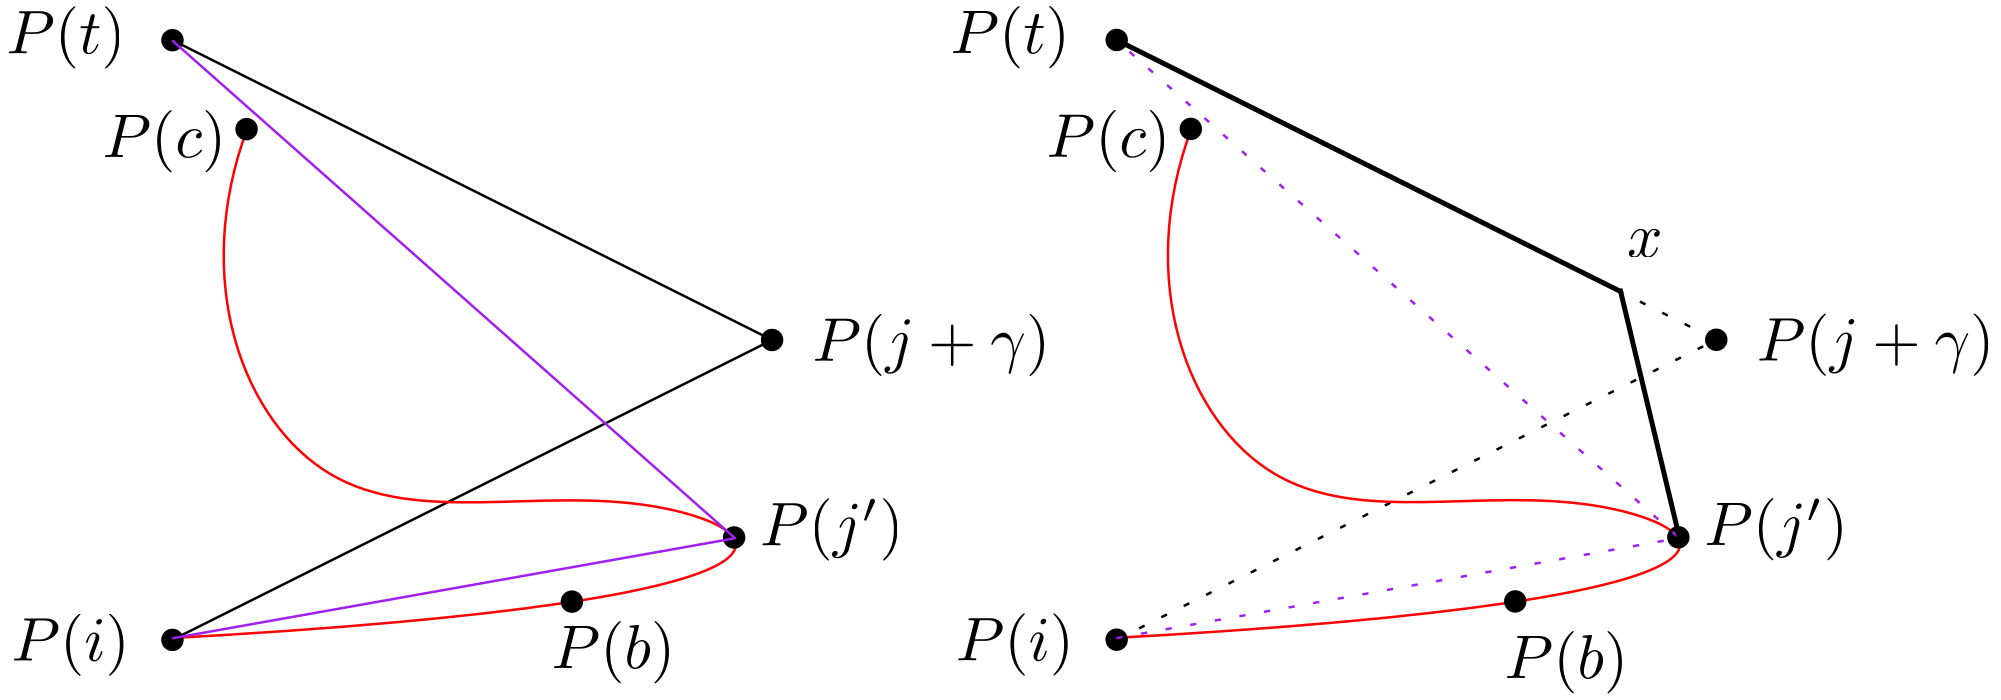
\includegraphics[scale=0.1]{./figures/case2.png}
		\caption{Case 2. Showing \(\delta^F(P[j' \dots c], \overline{P(j')P(t)}) \leq \varepsilon\) using \(\delta^F(P[j' \dots c], \overline{xP(t)}) \leq \varepsilon\) and \(P(j') - \varepsilon \leq x \leq P(j')\).}
		\label{fig:case2}
	\end{figure}

	For the first statement, we differentiate two cases.

	\paragraph{Case 2.1: \(P(b) > P(j')\)} 
	This case cannot occur as \(j' > b\) so both endpoints of the line segment that contains \(b\) are in the subpolyline \([i, c]\) and thus considered for the definition of \(j'\).

	\paragraph{Case 2.2: \(P(b) \leq P(j')\)} 
	Refer to \cref{fig:case22}. No point on the subpolyline \([i, j']\) is right of \(P(j')\) so we can use the same traversal as used in \(\overline{P(i)P(j+\gamma)}\) but stop when we reach \(\max(P(j')-\varepsilon, P(i))\). No point on the subpolyline requires a point further right than \(P(j')\) so \(P(j')-\varepsilon\) is the rightmost point we actually need to go to on the shortcut to reach \(b\) on the polyline. Then we use the traversal from \(\overline{P(j+\gamma)P(t)}\) to go to \(j'\). This is possible because no point on \([b, j']\) can be left of \(P(j')-\varepsilon\) as the shortcut goes left but must match \(P(j')\) at some point. Then we finally go right to \(P(j')\) on the shortcut.

	\begin{figure}[b]
		\centering
		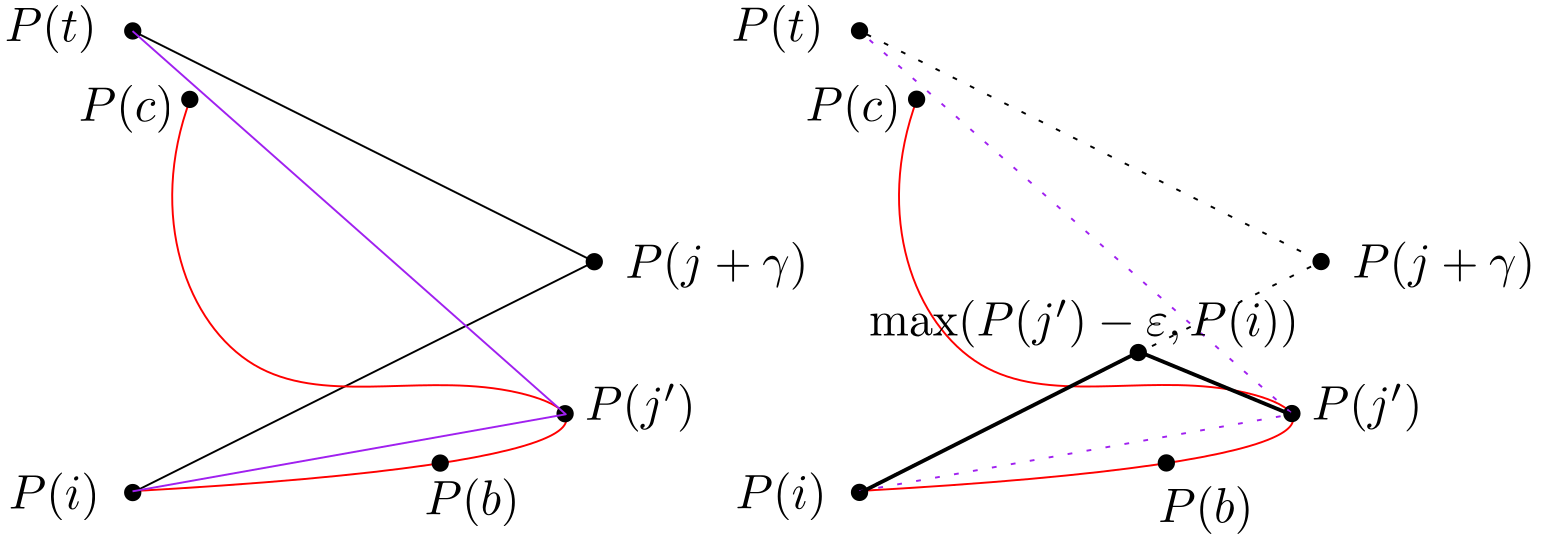
\includegraphics[scale=0.15]{./figures/case2-2.png}
		\caption{Case 2.2. Showing \(\delta^F(P[i \dots j'], \overline{P(i)P(j')}) \leq \varepsilon\) using \(\delta^F(P[i \dots b], \overline{P(i)x}) \leq \varepsilon\) and \(\delta^F(P[b \dots j'], x) \leq \varepsilon\) with \(x = \max(P(j')-\varepsilon, P(i))\).}
		\label{fig:case22}
	\end{figure}

	Iterating this procedure transforms the simplification to a local vertex-restricted one concluding the proof.
\end{proof}

\begin{corollary}\label{cor:local_extremal}
	Every one dimensional polyline has a local vertex-restricted simplification \(Q\) in which consecutive shortcuts \(e=\overline{uv}\) and \(e'=\overline{vw}\) satisfy that if \(e\) goes right then \(P(v)\) is rightmost in \([u, w]\) and if \(e\) goes left then \(P(v)\) is leftmost in \([u, v]\).
\end{corollary}

\begin{proof}
	The proof of \cref{thm:restr_frechet_1} constructs a local simplification that almost has this property. For a rightgoing shortcut \(\overline{uv}\) the construction guarantees that the end vertex is rightmost among the underlying subpolyline \([u, v]\). To also achieve the it is rightmost among the following shortcut \(\overline{vw}\), we determine the rightmost vertex in the combined subpolyline \([u, w]\) and make it the new end vertex \(v'\). The proof that that still yields local shortcuts is a simplified version of Case 1 or Case 2.2. This process can affect the vertices \(u\) and \(w\) which may need further updates in the same way (but in the other direction) but the process must stop at some point as each time we lengthen two shortcuts while all other shortcuts are unchanged. Only finitely many local simplifications can exist and this process strictly increases the total length of the shortcuts. Thus, we must reach some maximal simplification which has the stated property.
\end{proof}

\begin{corollary}\label{cor:frechet1dall}
	All five Fréchet variants can be solved in linear time in \(\R^1\).
\end{corollary}

\begin{proof}
	The proof from \cref{thm:restr_frechet_1} gives a linear time algorithm to transform curve-restricted global simplifications to local vertex-restricted ones in linear time and shows that all four restricted cases have the same size. A curve-restricted simplification can be computed using the algorithm from \citeauthor{global_curve_simplification}. 

	The final case is the unrestricted case. We transform an unrestricted simplification to a restricted one. We can assume that all points of the simplification actually lie on the polyline (although not necessarily in order) because if the lie outside the total range of the polyline we can move the respective points to the nearest extremal point on the polyline as no point on the polyline requires going that away. We can reexamine the proof of \cref{thm:restr_frechet_1} and note that we actually do not need that \(i < j + \gamma < t\) as we only argued using the position of \(P(j+\gamma)\) not its index.
\end{proof}

\subsection{Local Simplification in Linear Time}
Although this already yields a simplification algorithm in linear time for all four restricted settings, we present a simple linear time algorithm that directly computes a local vertex-restricted simplification (and thus a simplification for all four restricted settings). The same algorithm can be adapted to the Hausdorff distance with minor changes.

\begin{theorem}
	A local vertex-restricted Fréchet simplification can be computed in \(\O(n)\) using a greedy algorithm.

	A local vertex-restricted Hausdorff (undirected and directed from the polyline to the simplification) simplification can be computed in \(\O(n)\) using a greedy algorithm.
\end{theorem}

\begin{proof}
	We use \cref{cor:local_extremal} (the proof of this in the Hausdorff case mostly the same but simpler because we only need to consider the nearest points) to restrict the search space.

	We start with the first polyline vertex \(u_0\) and determine the first vertex \(v\) with \(|u_0-v| > \varepsilon\).

	\paragraph{Claim: If \(v\) is right of \(u_0\) the first shortcut goes right and otherwise left. } Without loss of generality assume \(v\) is right of \(u_0\), i.e., \(P(v) > P(u_0) + \varepsilon\). There can be no local shortcut to a vertex \(v'\) with \(P(v') + \varepsilon < P(u_0)\) as the shortcut must traverse \(v\) before but no point on the shortcut is within \(\varepsilon\) of \(v\). Otherwise \(P(u_0) - \varepsilon \leq P(v') \leq P(u_0)\). The following shortcut must go right by the \cref{lem:zigzag}. If \(\overline{v'w}\) is such a right-going shortcut then \(\overline{u_0w}\) is also one that covers the same polyline but is shorter. This is because we can go on the polyline from \(u_0\) to \(v'\) without needing to move from \(u_0\) as all points between are within distance \(\varepsilon\) if \(u_0\). After this, we use the local shortcut \(\overline{v'w}\) while never going left which is possible as no point is left of \(P(u_0)-\varepsilon\).

	With this, the direction of the first shortcut is known and thus the direction of all shortcuts (if no point leaves the boundary \([P(u_0) - \varepsilon, P(u_0) + \varepsilon]\) the shortcut from start to end is local as we can traverse the whole polyline without moving from the start and then just go to the end on the shortcut). Suppose the next shortcut that we need to construct goes right. We can traverse the polyline and only consider the newest rightmost vertices found. If any point found is left of the last rightmost vertex, we do not need to consider it by \cref{cor:local_extremal}. Let \(v\) be the current rightmost vertex found as we iterate then the shortcut can be extended to the next vertex as long as the next vertex is right of \(P(v) - \varepsilon\). If it would be left of that the shortcut cannot reach the previous vertex \(v\). Thus for vertex \(u\), the set of end vertices for a following shorcut is \(\set{u+1, \dots, k}\) where \(k\) is the first vertex that is more than \(\varepsilon\) to the left of the rightmost vertex in that range (in the case of the Hausdorff distance, we need to compare against \(P(u) - \varepsilon\) instead as going right extends the range but going left leaves it and every point of the polyline is close to some point on the simplification and the other way around).

	We finally argue that we can actually always go to the rightmost vertex for the shortcut. Consider the following shortcut for this. If it is after the rightmost vertex, we use \cref{cor:local_extremal}. Otherwise the following shortcut goes to a vertex before the rightmost one. Such a shortcut can be replaced by a direct shortcut to the end of the second shortcut as we have already argued that it must be a valid local shortcut.

	With this the algorithm for both Fréchet and Hausdorff can be described as a simple greedy algorithm: Find the first vertex outside of \(\varepsilon\) of the start and this determines the direction which is right (left). Then go to the rightmost (leftmost) vertex possible while maintaining the left (right) boundary that when exceeded disqualifies all further shortcuts. In the Fréchet case the left boundary is updated as \(P(v) - 2\varepsilon\) where \(v\) is the rightmost vertex currently found (or \(P(v) + 2\varepsilon\) for the right boundary when going left) because we can wait on the shortcut to the rightmost (leftmost) point with a distance of \(\varepsilon\) which covers everything \(2\varepsilon\) to the left of the rightmost (leftmost) vertex. In the Hausdorff case this boundary never needs to change and remains at \(P(u) - \varepsilon\) for the left boundary (or \(P(u) + \varepsilon\) for the right boundary) where \(u\) is the vertex from which we want to find the next shortcut. If at any point a shortcut to the end is possible we just go there. If we exceed the boundary, we add the rightmost (leftmost) vertex, change direction and repeat. Pseudocode for both variant can be found in \cref{algo:frechet1d,algo:hausdorff1d}; here \(1\) is right and \(-1\) is left and use the sign function sgn. 
\end{proof}

\begin{algorithm}[htb]
  \DontPrintSemicolon
	\KwData{One dimensional Polyline \(P\) of length \(n\), \(\varepsilon \geq 0\)}
	\KwResult{Local vertex-restricted Fréchet simplification \(Q\)}
  \BlankLine
	Let \(i\) be minimal with \(|P(i)-P(0)| > \varepsilon\) or \(n+1\) if it does not exist. 

	Let dir \(\gets\) sgn(\(P(i)-P(0)\)).

	\(Q = \angl{P(0)}\)\;
	extremal \(\gets P(i)\)\;
	\For{\(j = i\) \KwTo \(n\)}{
		\If{\((P(j) - P(\textrm{extremal})) \cdot \textrm{dir} > 0\)}{
			extremal \(\gets j\)
		} \ElseIf{\((P(\textrm{extremal}) - P(j)) \cdot \textrm{dir} > 2\varepsilon\)}{
			\(Q\).append(extremal)\;
			extremal \(\gets j\)\;
			dir \(\gets -\textrm{dir}\)
		}
	}
	\Return \(Q + \angl{P(n)}\)
	\caption{OneDimensionalFrechetSimplification(\(P\), \(\varepsilon\))}
  \label{algo:frechet1d}
\end{algorithm}

\begin{algorithm}[htb]
  \DontPrintSemicolon
	\KwData{One dimensional Polyline \(P\) of length \(n\), \(\varepsilon \geq 0\)}
	\KwResult{Local vertex-restricted Hausdorff simplification \(Q\)}
  \BlankLine
	Let \(i\) be minimal with \(|P(i)-P(0)| > \varepsilon\) or \(n+1\) if it does not exist. 

	Let dir \(\gets\) sgn(\(P(i)-P(0)\)).

	\(Q \gets \angl{P(0)}\)\;
	extremal \(\gets P(i)\)\;
	boundary \(\gets P(0) -\textrm{dir} \cdot \varepsilon\)\;
	\For{\(j = i\) \KwTo \(n\)}{
		\If{\((P(j) - P(\textrm{extremal})) \cdot \textrm{dir} > 0\)}{
			extremal \(\gets j\)
		} \ElseIf{\((\textrm{boundary} - P(j)) \cdot \textrm{dir} > 0\)}{
			\(Q\).append(extremal)\;
			dir \(\gets -\textrm{dir}\)\;
			boundary \(\gets P(j) -\textrm{dir} \cdot \varepsilon\)\;
			extremal \(\gets j\)
		}
	}
	\Return \(Q + \angl{P(n)}\)
	\caption{OneDimensionalHausdorffSimplification(\(P\), \(\varepsilon\))}
  \label{algo:hausdorff1d}
\end{algorithm}
\subsection{Conclusion}
This section is mostly theoretical as the most used setting is two dimensional simplification (although use cases for one dimensional simplification exist, e.g., \citeauthor{clustering_time_series}). The main practical consequence is that it demonstrates that in low dimensions it is definitely possible to achieve subcubic runtime.

We summarize our findings in \cref{thm:results1d}.
\begin{theorem}\label{thm:results1d}
  In \(\R^1\) polyline simplification using the Hausdorff and Fréchet distance has the following runtimes
	\begin{itemize}
		\item \(\O(n)\) for all Fréchet settings,
		\item \(\O(1)\) for all directed Hausdorff settings where the direction is from the simplification to the polyline,
		\item \(\O(n)\) for all other Hausdorff settings. If the leftmost and rightmost values are known in advance, all global settings can be computed in \(\O(1)\).
	\end{itemize}
\end{theorem}

\begin{proof}
	The five Fréchet cases are covered in \cref{cor:frechet1dall}. For the directed Hausdorff distance from the simplification to the Polyline, note that the shortcut from start to end always has distance 0 as each point in the simplification lies between the start and end and the polyline must contain every point in that range. 

	The remaining six global Hausdorff cases are trivial to solve. A simplification containing the leftmost and rightmost vertex as well as the start and end always has distance 0. It is trivial to test if the leftmost and rightmost vertices are needed in the simplification by testing if they lie within \([P(0) - \varepsilon, P(n) + \varepsilon]\) if \(P(0) \leq P(n)\) or \([P(n) - \varepsilon, P(0) + \varepsilon]\) otherwise. If they lie in the range, we can skip them, otherwise we need them. All of this can be computed in constant time once the leftmost and rightmost vertices are known.

	Now, only four local Hausdorff cases remain. Note that in one dimension and using local vertex-restricted measurement, using undirected Hausdorff and directed from polyline to simplification is the same because the other direction always has distance 0 in the local case and thus is not the maximum in the computation of the undirected case. 

	We have a linear algorithm for the local cases in \cref{algo:hausdorff1d}. We now claim that the vertex-restricted simplification is also optimal in the curve-restricted setting. If only one shortcut is needed, this is trivial. Thus assume there are at least two shortcuts and let \(e = \overline{P(i)P(j+\gamma)}\) be the first non vertex-restricted local shortcut. If it is the last shortcut mirror the polyline. Otherwise there is a following local shortcut \(e' = \overline{P(j+\gamma)P(t)}\) and assume \(e\) goes right and \(e'\) goes left. We use the same idea and replace \(P(j+\gamma)\) with the rightmost vertex in \([i, t]\). If this does not contain \(P(j+1)\) then \(P(t)\) lies on the line segment \(\overline{P(j)P(j+1)}\) and thus must go right of \(P(j+\gamma)\). This contradicts that \(e'\) goes left. Thus both endpoints of \(P(j+\gamma)\) are in \([i, t]\). Replacing \(P(j+\gamma)\) with the rightmost vertex (which is at least one of the endpoints of \(P(j+\gamma)\)) results in valid local shortcuts because of the simple nature of the Hausdorff distance as we have extended the shortcut to cover exactly the underlying polyline and no order needs to be considered.
\end{proof}

This solves the complexity problem for 20 out of the 30 settings in \citeauthor{global_curve_simplification}. The only ones missing are the five discrete Fréchet settings and the five weak Fréchet settings. Interestingly, in all cases, the vertex-restricted simplification is a curve-restricted simplification. We speculate that this is also the case for the other two settings, as the core geometric constraints of the one-dimensional line likely impose similar structural properties on their optimal simplifications.
